\chapter{Bayes Theorem}
\label{ch:bayes_theorem}

\section{What is Bayes Theorem ?}
Bayes theorem is what allows us to go from a sampling (or likelihood) distribution and a prior distribution to a posterior distribution.

A sampling distribution is the probability of seeing our data ($X$) given our parameters ($\theta$). This is written as $p(X|θ)$.

For example, we might have data on 1,000 coin flips. Where 1 indicates a head. This can be represented in python as
\begin{ipython}
import numpy as np

data_coin_flips = np.random.randint(2, size=1000)
np.mean(data_coin_flips)
\end{ipython}
\begin{ioutput}
0.495
\end{ioutput}

A sampling distribution allows us to specify how we think these data were generated. For our coin flips, we can think of our data as being generated from a Bernoulli Distribution. This distribution takes one parameter $p$ which is the probability of getting a 1 (or a head for a coin flip). It then returns a value of 1 with probablility $p$ and a value of 0 with probablility $(1-p)$.

You can see how this is perfect for a coin flip. With a fair coin we know our $p = .5$ because we are equally likely to get a 1 (head) or 0 (tail). 

This is a pretty simple PMF, but other distributions can get much more complicated. So it is good to know that Scipy has most of these built in. We can draw from the PMF as follows:

\begin{ipython}
from scipy.stats import bernoulli

print(bernoulli.pmf(1, .5))
print(bernoulli.pmf(0, .5))
\end{ipython}
\begin{ioutput}
0.5
0.5
\end{ioutput}

This is nice, but what we really want to know is the probability of see all 1000 of our data points. How do we do that? The trick here is to assume that our data are independent and identically distributed. This assumption allows us to say the probability of seeing all of our data is just the product of each individual probability: $p(x_1,\ldots,x_n|\beta)=p(x_1|\beta)\cdot\ldots\cdot p(x_n|\beta).$ This is easy to do:

\begin{ipython}
print (np.product(bernoulli.pmf(data_coin_flips, .5)))
\end{ipython}
\begin{ioutput}
9.3326361850321888e-302
\end{ioutput}

How does that number help us? Well by itself, it doesn't really help too much. What we need to do now is get more of a distribution for our sampling model. 

Currently, we have only tested our model with $p = .5$, but what if $p = .8$ ? or .2 ? What would the probablility of our data look like then ? 

This can be done by defining a grid of values for our $p$. Below I will make a grid of 100 values between 0 and 1 (because $p$ has to be between 0 and 1) and then I will calculate the probability of seeing our data given each of these values:
\begin{ipython}
import matplotlib.pyplot as plt

params = np.linspace(0, 1, 100)
p_x = [np.product(st.bernoulli.pmf(data_coin_flips, p)) for p in params]
plt.plot(params, p_x)
plt.show()
\end{ipython}

Now we are getting somewhere. We can see that the probablility of seeing our data peaks at $p=.5$ and almost certainly is between $p=.4$ and $p=.6$. 
So now we have a good idea of what $p$ value generated our data assuming it was drawn from a Bernoulli distribution. We’re done, right? Not quite\ldots

\subsubsection{Prior Distribution}
Bayes theorem says that we need to think about both our sampling distribution and our prior distribution. What do I mean by prior distribution? It is the $p(\theta)$ or the probability of seeing a specific value for our parameter. In our sampling distribution we defined 100 values from 0 to 1 for our parameter $p$. Now we must define the prior probability of seeing each of those values. That is the probability we would have assumed before seeing any data. Most likely, we would have assumed a fair coin, which looks like the distribution above. Lets see how we can do this:

\begin{ipython}
fair_flips = bernoulli_flips = np.random.binomial(n=1, p=.5, size=1000)
p_fair = np.array([np.product(st.bernoulli.pmf(fair_flips, p)) for p in params])
p_fair = p_fair / np.sum(p_fair)
plt.plot(params, p_fair)
\end{ipython}

Basically we created 1000 fair coin flips and then generated the sampling distribution like we did before (except we divided by the sum of the sampling distribution to make the values sum to 1). Now we have a “fair coin” prior on our parameters. This basically means that before we saw any data we thought coin flips were fair. And we can see that assumption in our prior distribution by the fact that our prior distribution peaks at .5 and is almost all between .4 and .6.
I know what you are thinking - this is pretty boring. The sampling and prior distributions look exactly the same. So lets mix things up. Lets keep our fair prior but change our data to be an unfair coin:

\begin{ipython}
unfair_flips = bernoulli_flips = np.random.binomial(n=1, p=.8, size=1000)
p_unfair = np.array([np.product(st.bernoulli.pmf(unfair_flips, p)) for p in params])
fig, ax = plt.subplots(2, 1, sharex=True)
ax[0].plot(params, p_unfair)
ax[0].set_title("Sampling Distribution")
ax[1].plot(params, p_fair)
ax[1].set_title("Prior Distribution")
plt.tight_layout()
plt.show()
\end{ipython}

Now this is interesting. We have strong data evidence of an unfair coin (since we generated the data we know it is unfair with $p=.8$), but our prior beliefs are telling us that coins are fair. How do we deal with this?

\subsection{Bayes Theorem (Posterior Distribution)}
Bayes theorem is what allows us to go from our sampling and prior distributions to our posterior distribution. The posterior distribution is the $P(\theta|X)$. Or in English, the probability of our parameters given our data. And if you think about it that is what we really want. We are typically given our data and we want to figure out what parameters are most likely given our data. So how do we get to this posterior distribution ? 
By definition, we know that:
\begin{itemize}
\item $P(A|B) = \dfrac{P(A,B)}{P(B)}$, the probability of seeing $A$ given $B$ is the probability of seeing them both divided by the probability of $B$;
\item $P(B|A) = \dfrac{P(A,B)}{P(A)}$, the probability of seeing $B$ given $A$ is the probability of seeing them both divided by the probability of $A$.
\end{itemize}

You will notice that both of these values share the same numerator, so:

$P(A,B) = P(A|B) P(B)$

$P(A,B) = P(A|B) P(B)$

Thus:

$P(A|B) P(B) = P(B|A) P(A)$

Which implies:

$P(A|B) = \dfrac{P(B|A) P(A)}{P(B)}$

And plug in $\theta$ for $A$ and $X$ for $B$:

$P(\theta|X) = \dfrac{P(X|\theta)*P(\theta)}{P(X)}$

Nice! Now we can plug in some terminology we know:

$Posterior = \dfrac{likelihood \cdot prior}{P(X)}$
But what is the $P(X)$, the probability of our data? 
That sounds weird\ldots Let’s go back to some math and use $B$ and $A$ again:

We know that $P(B)=\sum_A P(A,B)$

And from our definitions above, we know that:

$P(A,B) = P(A|B)\cdot P(A)$

Thus:

$P(B) = \sum_{A} P(A|B)\cdot P(A)$

Plug in our $\theta$ and $X$:

$P(X) = \sum_{\theta} P(\theta|X)*P(\theta)$

Plug in our terminology:

$P(X) = \sum_{\theta} likelihood \cdot prior$

Wow! Isn’t that awesome! But what do we mean by $\sum\theta$. This means to sum over all the values of our parameters. In our coin flip example, we defined 100 values for our parameter $p$, so we would have to calculated the $likelihood \cdot  prior$ for each of these values and sum all those anwers. That is our denominator for Bayes Theorem. Thus our final answer for Bayes is:

$Posterior = \dfrac{likelihood \cdot prior}{\sum_{\theta} likelihood \cdot prior}$

That was a lot of text. Let’s do some more coding and put everything together.

\begin{ipython}
def bern_post(n_params=100, n_sample=100, true_p=.8, prior_p=.5, n_prior=100):
  params = np.linspace(0, 1, n_params)
  sample = np.random.binomial(n=1, p=true_p, size=n_sample)
  likelihood = np.array([np.product(st.bernoulli.pmf(sample, p)) for p in params])
  #likelihood = likelihood / np.sum(likelihood)
  prior_sample = np.random.binomial(n=1, p=prior_p, size=n_prior)
  prior = np.array([np.product(st.bernoulli.pmf(prior_sample, p)) for p in params])
  prior = prior / np.sum(prior)
  posterior = [prior[i] * likelihood[i] for i in range(prior.shape[0])]
  posterior = posterior / np.sum(posterior)

  fig, ax = plt.subplots(3, 1, sharex=True, figsize=(8,8))
  ax[0].plot(params, likelihood)
  ax[0].set_title("Sampling Distribution")
  ax[1].plot(params, prior)
  ax[1].set_title("Prior Distribution")
  ax[2].plot(params, posterior)
  ax[2].set_title("Posterior Distribution")
  plt.tight_layout()
  plt.show()
  return posterior

example_post = bern_post()
\end{ipython}

You will notice that I set 100 as the number of observations for the prior and likelihood. This increases the variance of our distributions. More data typically decreases the spread of a distribution. Also, as you get more data to estimate your likelihood, the prior distribution matters less.

\begin{ipython}
moredata_post = bern_post(n_sample=1000)
\end{ipython}

You can see that effect in the graphs above. Because we have more data to help us estimate our likelihood our posterior distribution is closer to our likelihood.

You will notice that the denominator for Bayes Theorem is just a constant. So if you only want to get the maximum posterior value, you don’t even need to calculate that constant. For this reason you will often see the posterior shown as proportional to the $likelihood \cdot prior$.

\begin{figure}[h]
  \begin{center}
    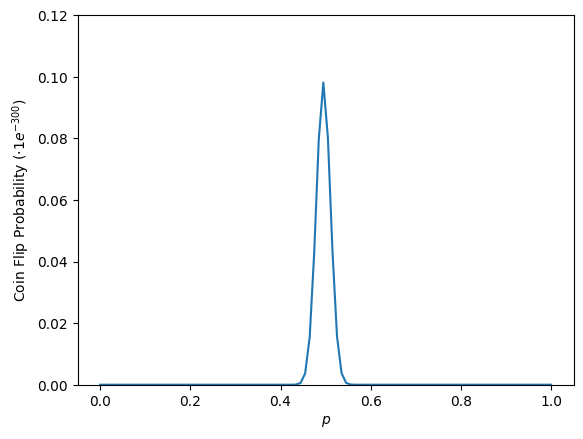
\includegraphics[width=0.6\linewidth]{figures/bayes_p1}
  \end{center}
  \caption{Prob}
  \label{fig:bayes_p1}
\end{figure}

\begin{figure}[h]
  \begin{center}
    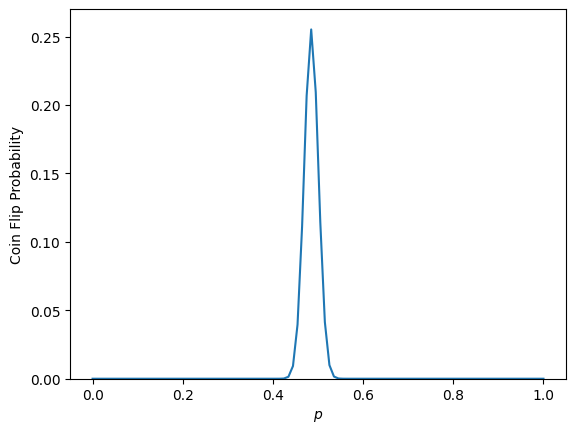
\includegraphics[width=0.6\linewidth]{figures/bayes_p2}
  \end{center}
  \caption{Prob}
  \label{fig:bayes_p2}
\end{figure}

\begin{figure}[h]
  \begin{center}
    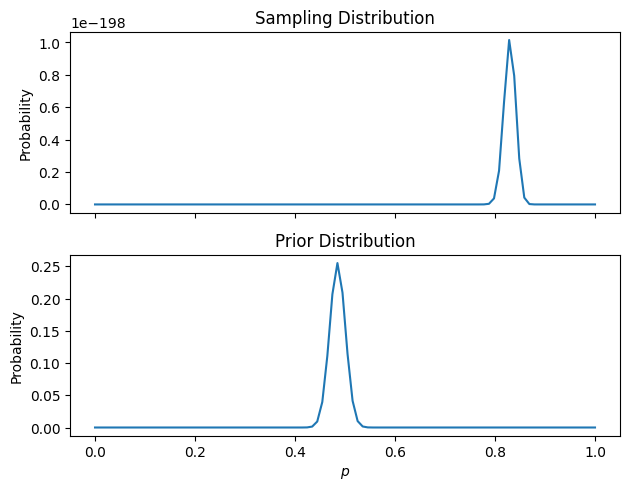
\includegraphics[width=0.6\linewidth]{figures/bayes_p3}
  \end{center}
  \caption{Prob}
  \label{fig:bayes_p3}
\end{figure}

\begin{figure}[h]
  \begin{center}
    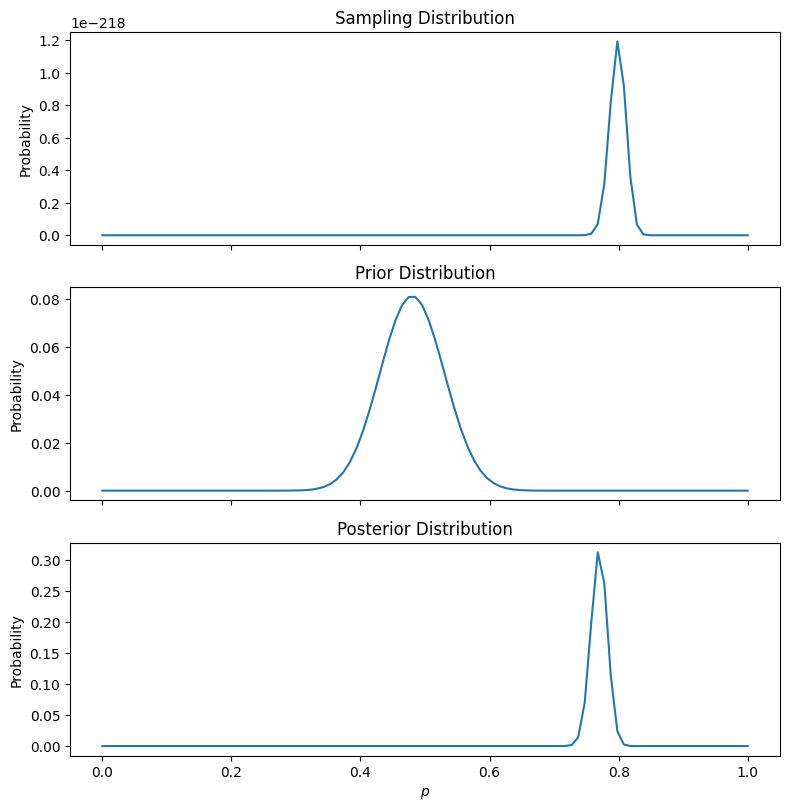
\includegraphics[width=0.6\linewidth]{figures/bayes_p5}
  \end{center}
  \caption{Prob}
  \label{fig:bayes_p5}
\end{figure}

\begin{figure}[h]
  \begin{center}
    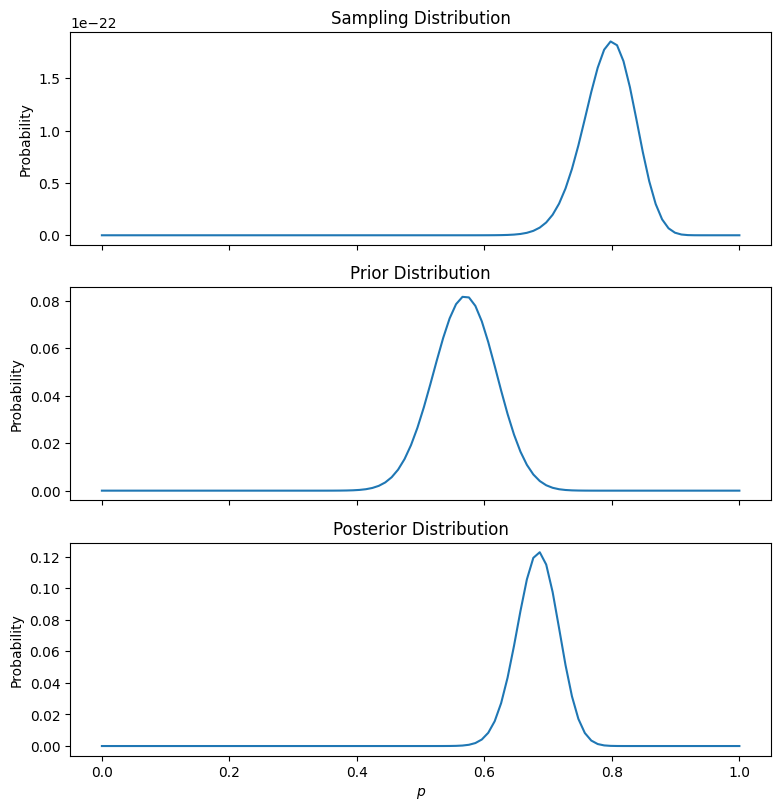
\includegraphics[width=0.6\linewidth]{figures/bayes_p4}
  \end{center}
  \caption{Prob}
  \label{fig:bayes_p4}
\end{figure}

%Frequentist statistics is focused on the likelihood. Or you could say that frequentists are bayesians with a non-informative prior (like a uniform distribution). But don’t hate on frequentists too much; most of bayesian inference in applied settings relies of frequentists statistics.
%Now that you know frequentist statistics focuses on the likelihood it is much clearer why people often misinterpret frequentist confidence intervals. 
%The likelihood is $P(X|\theta)$, or the probability of our data given our parameters. That is a bit wierd because we are given our data, not our parameters. What most frequentists models do is take the maximum of the likelihood distribution (or Maximum Likelihood Estimation (MLE)). Basically find what parameters maximize the probability of seeing our data. The important point here is that they are treating the data as random, so what the frequentist confidence interval is saying is that if you were to keep getting new data (maybe some more surveys) and calculate confidence intervals on each of these new samples, 95% of these samples would have confidence intervals that contain the true parameter you are trying to estimate.
